\documentclass{article}
\usepackage{amsmath}
\documentclass{article}
\usepackage{listings}
\usepackage{xcolor}
\usepackage{matlab-prettifier}
\usepackage{graphicx}
\usepackage{fancyhdr}
\usepackage[sorting=none]{biblatex}
\usepackage[margin=1in]{geometry}
\usepackage{listings}
\usepackage[hidelinks]{hyperref}
\usepackage{xcolor}
\usepackage{xepersian}
\addbibresource{bibliography.bib}
\settextfont[Scale=1.2]{B-NAZANIN.TTF}
\setlatintextfont[Scale=1]{Times New Roman}
\renewcommand{\baselinestretch}{1.5}
\pagestyle{fancy}
\fancyhf{}
\rhead{پروژه اول درس داده‌کاوی }
\lhead{\thepage}
\rfoot{ آیلین نائب‌زاده}
\lfoot{99522185}
\renewcommand{\headrulewidth}{1pt}
\renewcommand{\footrulewidth}{1pt}

\begin{document}
\begin{titlepage}
\begin{center}

\includegraphics[width=0.4\textwidth]{IUSTLogo.png}\\
        
\LARGE
\textbf{دانشگاه علم و صنعت ایران}\\
\textbf{دانشکده مهندسی کامپیوتر}\\
        
\vfill
        
\huge
\textbf{عنوان: پروژه چهارم درس داده‌کاوی}\\
\textbf{رتبه‌بندی ویژگی‌های مؤثر در دسته‌بندی مجموعه داده‌ها}\\
\vfill
        
\LARGE
\textbf{نام و نام خانوادگی: آیلین نائب‌زاده }\\
\textbf{شماره دانشجویی: 99522185}\\
\textbf{نیم‌سال تحصیلی: پائیز 1402}\\
\textbf{مدرّس: دکتر حسین رحمانی}\\
\end{center}
\end{titlepage}


\tableofcontents
\newpage

\section{گام اول}  
در طی این پروژه، باتوجه به اینکه داده‌های ما در پنج فایل مجزا قرار گرفته‌اند، در ابتدا نیاز است که جداگانه سعی کنیم محتوای هر یک از فایل‌ها را بشناسیم.
در اولین قدم با مراجعه به سایت \lr{Google Colab} و ساخت یک پروژه جدید و فراخوانی بعضی از کتابخانه‌های معروف زبان \lr{Python} شروع به مشاهده داده‌های موجود در هر فایل و انجام تحلیل‌های ابتدایی می‌کنیم.
لیست برخی کتابخانه‌های استفاده‌شده به‌همراه محیط کلی پروژه را در تصویر زیر می‌توانید مشاهده کنید.
\begin{figure}[ht]
        \centering
        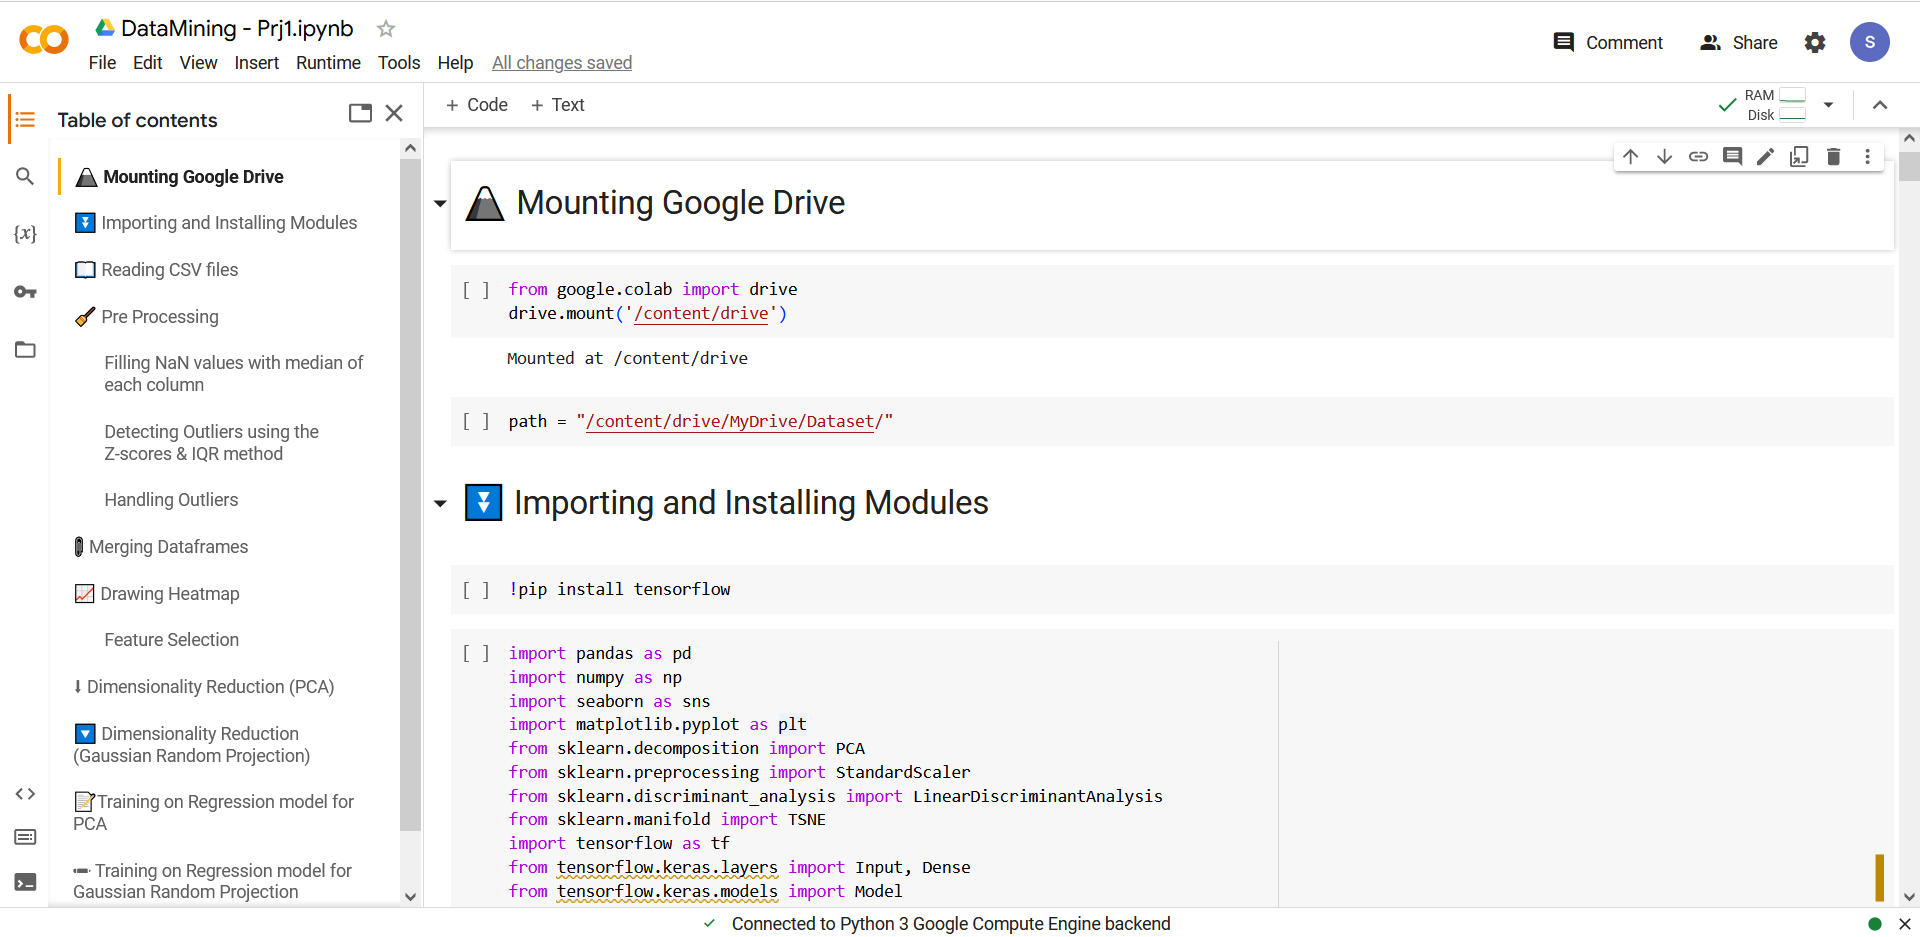
\includegraphics[width=1\textwidth]{project-1.png}
        \caption{نمای کلی از پروژه \lr{notebook} در فضای \lr{Google Colab}}
        \label{fig:fig1}
    \end{figure}

برای راحتی کار و سرعت بیشتر، فایل‌های موجود در پوشه \lr{Dataset} را در \lr{Google Drive} می‌توانیم آپلود کنیم و سپس بااستفاده از دستور \lr{google.mount} و تعریف مسیر درست، به‌راحتی به فایل‌ها دسترسی داشته‌ باشیم.
در ادامه برای خواندن فایل‌های \lr{csv} و \lr{excel} و تبدیل آن‌ها به شیء‌هایی از نوع \lr{dataframe} از توابع آماده و از پیش‌ تعریف شده \lr{read\_csv} و \lr{read\_excel} که در کتابخانه \lr{pandas} موجود هستند، استفاده می‌کنیم.

\newpage
همچنین در حین خوانش هر یک از فایل‌ها، می‌توانیم مواردی مانند نام ستون‌های موجود در هر فایل، تعداد مقادیر صفر در هر ستون، تعداد مقادیر تعریف نشده(\lr{NaN}) و درصد این‌گونه موارد به کل را حساب کنیم. بطور مثال گونه‌ای از این تحلیل‌ها را برای فایل \lr{demographic.csv} در تکه کد زیر می‌توانید مشاهده کنید.

\lr{\lstinputlisting[frame=single,
    numbers=left,
    style=Python,
    showstringspaces=false,
    basicstyle=\ttfamily,
    backgroundcolor=\color{gray!20!white},
    breaklines=true]{step1.py}}

\newpage
\section{گام دوم}
در مرحله پیش پردازش داده از روش‌های مختلفی می‌توانیم بهره ببریم. 

در ابتدا برای هر یک از فایل‌ها و ستون‌های موجود در آن‌ها می‌توانیم باتعریف یک حد آستانه مشخص کنیم که ستون‌هایی که تعداد مقادیر \lr{NaN} در آن‌ها از آن حد بیشتر باشد، حذف شوند.
سپس طبق توضیحات موجود در فایل پروژه به‌دنبال مقادیر ترکیب از ۷ و ۹ می‌گردیم و آن‌ها را با \lr{NaN} جایگزین می‌کنیم و مجددا مرحله قبل را تکرار می‌کنیم. در ادامه باتوجه به اینکه مقادیر \lr{SEQN} نقشی همانند \lr{Primary Key} در فایل‌های ما دارند، چک می‌کنیم که در یک فایل، دو یا بیش از دو \lr{SEQN} یکسان وجود نداشته باشد و درصورت وجود نیز تنها اولین نمونه آن را نگه می‌داریم.

در مرحله بعدی مقادیر \lr{NaN} باقی مانده را، با \lr{median} همان ستون خاص جایگزین می‌کنیم، چراکه این مقدار نسبت به \lr{Outlier}ها نیز حساس نمی‌باشد.

در نهایت برای شناسایی مقادیر \lr{Outlier} در هر فایل و در هر ستون آن‌ها، از روش \lr{IQR} استفاده می‌کنیم. البته روش‌های دیگری نیز همانند \lr{Z-Score} وجود دارند ولی همانطور که در فایل پروژه می‌توانید مشاهده کنید، روش \lr{IQR} تعداد \lr{Outlier}های بیشتری را شناسایی کرده‌است.

درنهایت پس از شناسایی \lr{Outlier}ها، آن‌ها را نیز با میانه موجود در هر ستون جایگزین می‌کنیم.
یکی از چالش‌ها و نکاتی که در این مرحله متوجه شدم، وجود مقادیری همچون \lr{P}، \lr{S} و ... بود که به ما اجازه تشخیص مقادیر \lr{Outlier} را نمی‌دادند. و در نتیجه نیاز بود تا در ابتدا مقادیر از نوع \lr{str} را نیز به حالت عددی در بیاوریم و به هر یک از آن مقادیر یک کد منحصر به‌فرد اختصاص دهیم.
\newpage
\section{گام سوم}
در گام سوم و برای تشخیص ویژگی‌های مهم‌تر در ابتدا تمامی فایل‌ها بجز فایل \lr{questionnaire.csv} را با یکدیگر مرج میزنیم. همچنین باید دقت کنیم که تمامی این عملیات براساس ویژگی \lr{SEQN} صورت می‌‌گیرد.
سپس بااستفاده از تابع \lr{.corr()} موجود در کتابخانه \lr{pandas} همبستگی بین دوبه‌دوی ویژگی‌ها را بدست می‌آوریم. سپس بااستفاده از توابعی مانند \lr{.abs} و \lr{.sort} سعی می‌کنیم صد جفت ویژگی که با هم بیشترین همبستگی را براساس اندازه مقدار \lr{Correlation Coefficient} دارند را برگردانیم.

البته به این نکته هم دقت می‌کنیم که جفت ویژگی‌هایی که بین یک ویژگی و خودش هست را در نظر نگیریم.
همچنین برای نمایش میزان همبستگی بین ویژگی‌ها و درک روابط بین صد ویژگی استخراج شده، از توابع موجود در کتابخانه \lr{matplotlib} و \lr{seaborn} استفاده می‌کنیم.

تصویر مربوط به نمودار نقشه حرارتی صد ویژگی استخراج شده را در تصویر زیر می‌توانید مشاهده کنید.

\begin{figure}[ht]
        \centering
        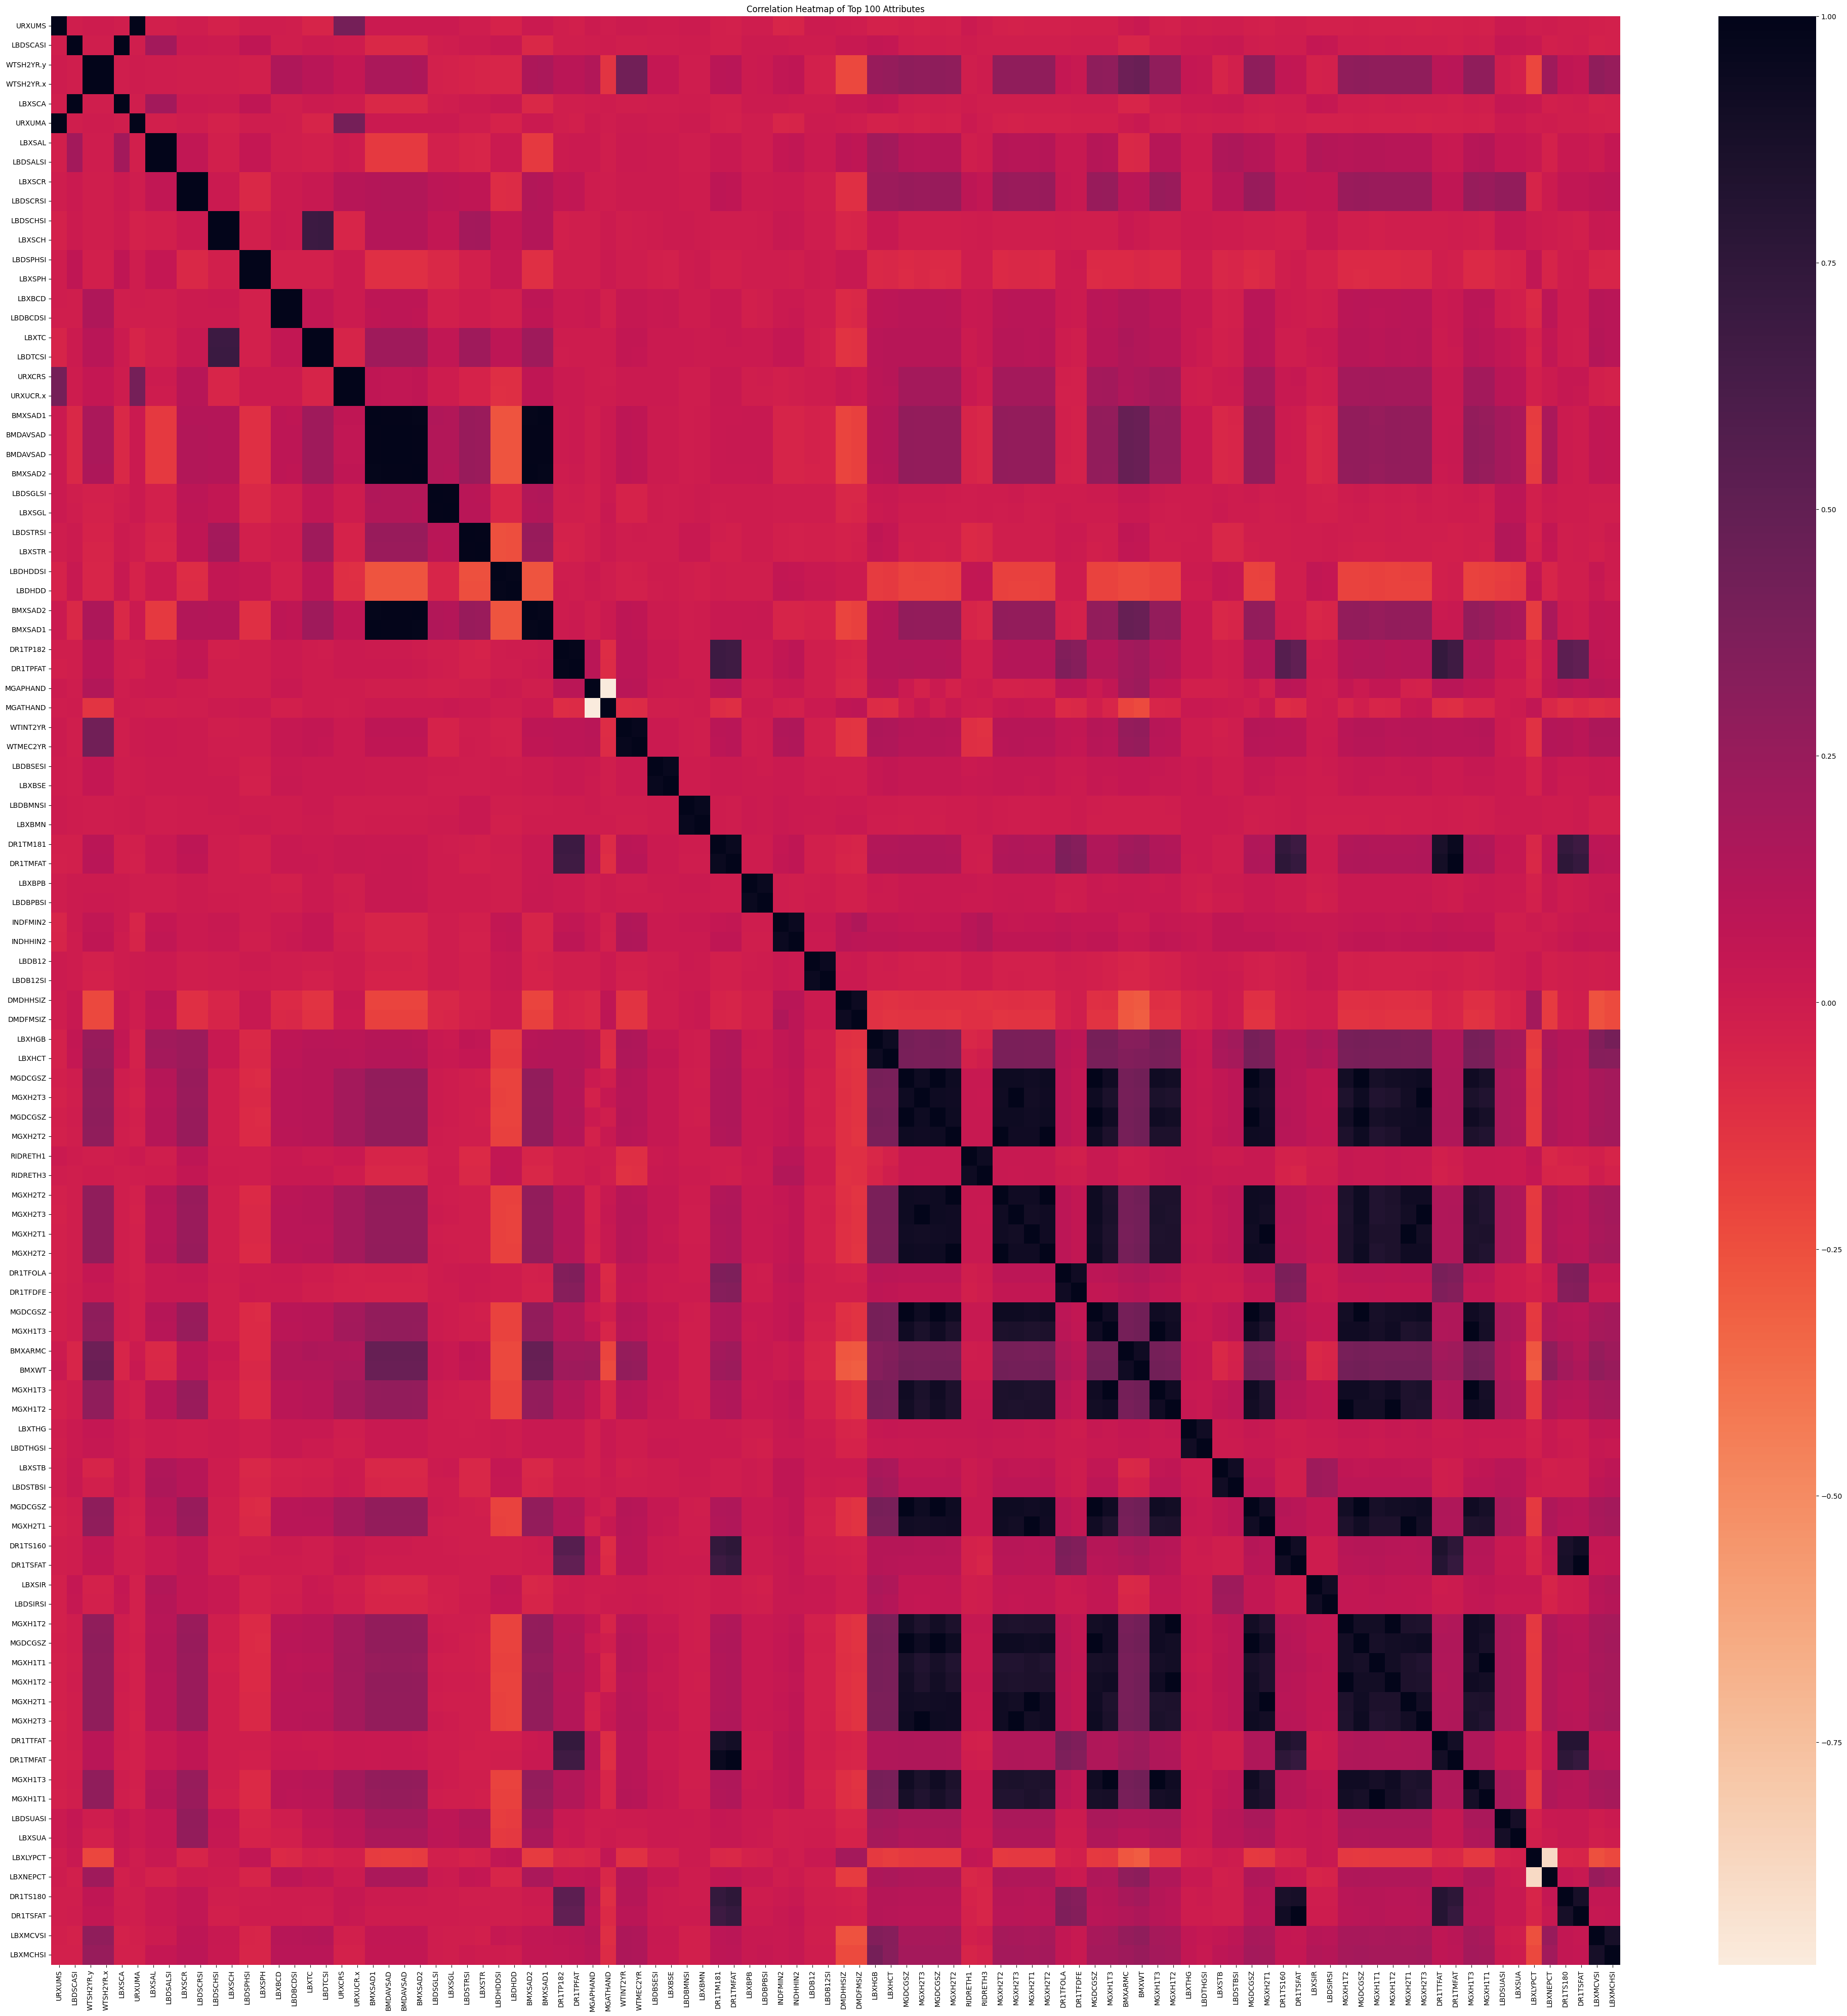
\includegraphics[width=0.7\textwidth]{heatmap.png}
        \caption{نمودار نقشه حرارتی صد ویژگی با بیشترین همبستگی}
        \label{fig:fig2}
\end{figure}

در نهایت برای انتخاب تنها یک ویژگی از میان ویژگی‌هایی که بیشترین همبستگی را با یکدیگر دارند، با تعریف یک حد آستانه(در این پروژه 8.0) ویژگی‌هایی که بیشترین ارتباط را با یکدیگر دارند در ابتدا در یک مجموعه ذخیره می‌کنیم و سپس اولین عضو آن‌ها را انتخاب می‌کنیم.
\newpage
\section{گام چهارم}
در این مرحله باتوجه به آرایه \lr{selected\_features} که تعریف کرده بودیم و توابع آماده موجود در کتابخانه \lr{sklearn} همانند \lr{PCA} سعی می‌کنیم تا ابعاد داده‌های خود را کاهش دهیم. همچنین پیش از استفاده از ماژول \lr{PCA} در ابتدا سعی می‌کنیم با استفاده از ماژول \lr{StandardScalar} داده‌های خود را نرملایز کنیم.
همچنین می‌توانیم با تغییر مقدار \lr{n\_components} تعداد کامپوننت‌هایی که می‌خواهیم داده‌های خود را به آن‌ها تقسیم کنیم، مشخص کنیم.

روش‌های بسیار دیگری برای کاهش ابعاد داده‌ها وجود دارند. باتوجه به نوع داده‌های مسئله، از ماژول \lr{GaussianRandomProjection} به‌عنوان روش دوم برای کاهش ابعاد استفاده کردم.

\newpage
\section{گام پنجم}
در مرحله پنجم باتوجه به خواسته مسئله که استفاده از خروجی‌های مرحله پیشین و آموزش مدل‌های \lr{Regression} بااستفاده از آن‌ها می‌باشد، می‌توانیم از مدل‌های \lr{Regression} موجود در کتابخانه \lr{sklearn} استفاده کنیم.
در این بخش سه مدل \lr{LinearRegression}، \lr{KNeighborsRegressor} و \lr{DecisionTreeRegressor} را برای داده‌های کاهش یافته از هر دو حالت \lr{PCA} و \lr{Gaussian Random Projection} در نظر می‌گیریم.

همچنین پیش از استفاده از این دو مدل، نیاز است که دیتاست مقادیر ورودی(\lr{X}) و لیبل(\lr{y}) خود را تعریف کنیم. دیتاست مقادیر ورودی درواقع داده‌های کاهش یافته می‌باشند و دیتاست لیبل‌ها نیز یک بار آرایه‌ای از مقادیر ابتلا/عدم ابتلا به سرطان و بار دیگر آرایه‌ای از ابتلا/عدم ابتلا به مشکلات کبدی می‌باشد.

همچنین باتوجه به اینکه تعداد ردیف‌های دو دیتاست داده‌های ورودی و مقادیر خروجی(لیبل‌ها) نیز باید یکسان باشد، باید تنها ردیف‌هایی از دیتاست لیبل‌ها را انتخاب کنیم که \lr{SEQN} آن‌ها در \lr{dataframe} تجمیع شده‌ای که بااستفاده از آن داده‌های کاهش یافته را ساختیم، موجود باشد.

سپس بااستفاده از تابع \lr{train\_test\_split} داده‌های ورودی خود را به یک نسبت دلخواه به دیتاست تست و آموزشی تجزیه می‌کنیم. 

در نهایت بااستفاده از دو تابع \lr{.fit} و \lr{.predict} مدل‌های خود را آموزش می‌دهیم و از آن‌ها برای پیش‌بینی مقادیر دیتاست تست استفاده می‌کنیم.

بطور مثال در صورتی که از داده‌های خروجی الگوریتم \lr{PCA} و لیبل‌های سرطانی بخواهیم استفاده کنیم کد پیاده‌سازی شده بصورت زیر می‌شود.

\lr{\lstinputlisting[frame=single,
    numbers=left,
    style=Python,
    showstringspaces=false,
    basicstyle=\ttfamily,
    backgroundcolor=\color{gray!20!white},
    breaklines=true]{step2.py}}

\newpage
\section{گام ششم}
در گام آخر می‌توانیم با معیارهایی همانند \lr{Mean Squared Error} و \lr{Mean Absolute Error} مدل خود را ارزیابی کنیم. نتایج مربوط به این ارزیابی را در چهار تصویر زیر می‌توانید مشاهده کنید.

\begin{figure}[ht]
        \centering
        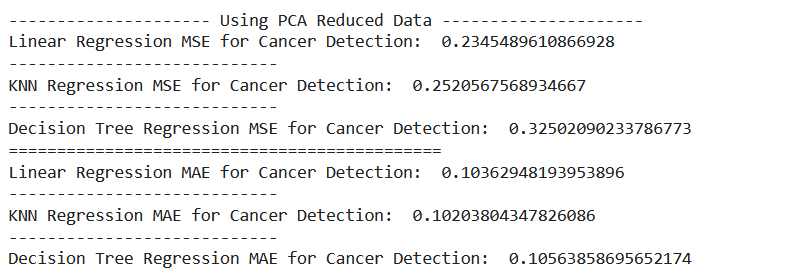
\includegraphics[width=0.7\textwidth]{pca-cancer.png}
        \caption{خروجی میزان ارور(خطا) در حالت استفاده از الگوریتم \lr{PCA} و برای داده‌های سرطانی}
        \label{fig:fig3}
\end{figure}

\begin{figure}[ht]
        \centering
        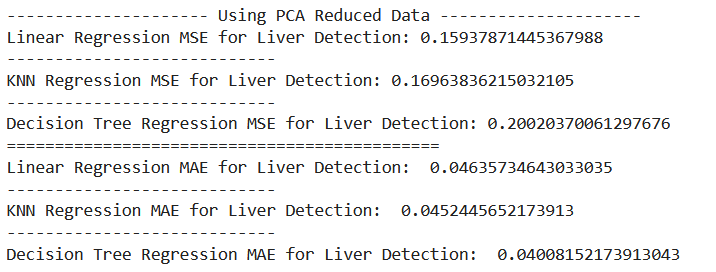
\includegraphics[width=0.7\textwidth]{pca-liver.png}
        \caption{خروجی میزان ارور(خطا) در حالت استفاده از الگوریتم \lr{PCA} و برای داده‌های کبدی}
        \label{fig:fig4}
\end{figure}

\newpage
\begin{figure}[ht]
        \centering
        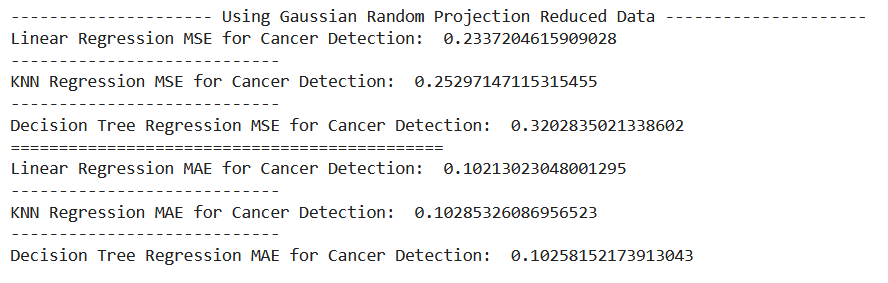
\includegraphics[width=0.7\textwidth]{gau-cancer.png}
        \caption{خروجی میزان ارور(خطا) در حالت استفاده از الگوریتم \lr{GRP} و برای داده‌های سرطانی}
        \label{fig:fig5}
\end{figure}

\begin{figure}[ht]
        \centering
        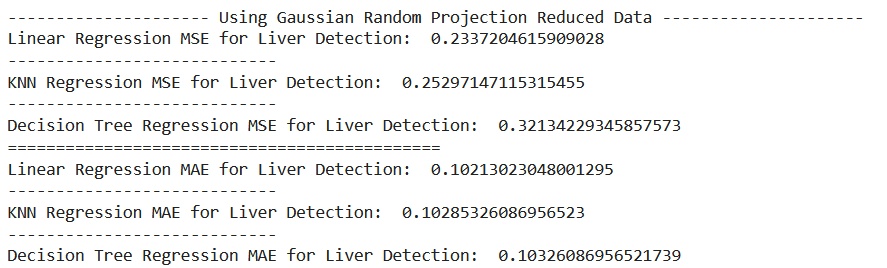
\includegraphics[width=0.7\textwidth]{gau-liver.png}
        \caption{خروجی میزان ارور(خطا) در حالت استفاده از الگوریتم \lr{GRP} و برای داده‌های کبدی}
        \label{fig:fig6}
\end{figure}

\newpage
\section{نتیجه‌گیری}
\subsection{نتیجه ارزیابی‌ها با روش \lr{PCA} و روش انتخابی خود}
در حالتی که لیبل‌های سرطانی را بررسی کرده باشیم، میزان ارور برگردانده‌شده در دو حالت استفاده از الگوریتم \lr{PCA} و \lr{GRP} بسیار شبیه به هم خواهد شد. ولی در صورتی که بخواهیم لیبل‌های مشکلات کبدی را بررسی کنیم، میزان ارور یا خطای برگردانده‌شده بااستفاده از الگوریتم \lr{PCA} به نسبت کمتر از حالتی خواهد شد که از الگوریتم \lr{GRP} استفاده کرده باشیم.
\subsection{تاثیرات انتخاب ویژگی‌ها - مزایا و معایب}
بله قطعا باتوجه به حجم بالای داده و تعداد بسیار زیاد ویژگی‌ها که به بیش از 500 می‌رسید، فیلتر ویژگی‌ها و انتخاب بعضی از آن‌ها سرعت اجرای بعضی از الگوریتم‌ها را افزایش می‌دهد. ولی باید به این نکته نیز توجه داشته باشیم که همواره حذف بعضی از ویژگی‌ها می‌تواند به معنی از دست رفتن اطلاعات نیز باشد. همچنین در صورت وجود تعداد بالای ویژگی‌ها تحلیل مدل‌ها و تفسیرپذیری آن‌ها نیز کاهش می‌یابد.

\subsection{مقایسه ویژگی‌های سرعت و دقت در دو مدل مختلف}
بطور کلی می‌توانیم بگوئیم \lr{PCA} معمولا صحت بیشتری دارد ولی به مدت زمان بیشتری برای اجرا احتیاج دارد. درصورتی که الگوریتم \lr{GRP} صحت کمتری دارد ولی سریع‌تر عمل می‌کند. ولی همچنان نمی‌توانیم نظر قطعی بدهیم و تمامی این موارد و معیارهای این چنینی وابسته به نوع داده‌های ورودی و مسئله هستند. چرا که بطور مثال سرعت و دقت \lr{PCA} وابسته به تعداد ویژگی‌ها و تعداد \lr{component}های مشخص شده دارد.
\end{document}
